\chapter{KEGIATAN KERJA PRAKTEK DAN PEMBAHASAN KRITIS}
\section{Kegiatan Bangkit 2022}
Bangkit 2022 dilaksanakan sepenuhnya secara daring, dengan pembelajaran sinkron melalui Google Meet, pembelajaran asinkron melalui Dicoding, Coursera, dan Qwiklabs, serta media koordinasi dan komunikasi melalui Google Classroom dan Discord. Kegiatan pembelajaran dilaksanakan selama 21 Minggu dari 14 Februari 2022 hingga 15 Juli 2022 dan dibagi menjadi beberapa modul.

\begin{longtable}{|p{2cm}p{2cm}|p{2cm}p{2cm}p{2cm}p{2cm}|}
	\hline
	\multicolumn{2}{|p{1cm}|}{Minggu ke-} &
	\multicolumn{1}{p{2cm}|}{Modul \textit{Soft Skill}} &
	\multicolumn{1}{p{2cm}|}{Modul \textit{English}} &
	\multicolumn{1}{p{2cm}|}{Modul \textit{Cloud Computing (Asynchronous)}} &
	Modul \textit{Cloud Computing (Synchronous)} \\ \hline
	\endfirsthead
	%
	\endhead
	%
	\multicolumn{1}{|p{1cm}|}{0} &
	7 Feb &
	\multicolumn{1}{p{2cm}|}{} &
	\multicolumn{1}{p{2cm}|}{English Pre-test} &
	\multicolumn{1}{p{2cm}|}{Matrikulasi} &
	\\ \hline
	\multicolumn{1}{|p{1cm}|}{1} &
	14 Feb &
	\multicolumn{1}{p{2cm}|}{} &
	\multicolumn{1}{p{2cm}|}{} &
	\multicolumn{1}{p{2cm}|}{Dicoding: Web Development Basics} &
	\\ \hline
	\multicolumn{1}{|p{1cm}|}{2} &
	21 Feb &
	\multicolumn{1}{p{2cm}|}{Pre-read: Time Management} &
	\multicolumn{1}{p{2cm}|}{} &
	\multicolumn{1}{p{2cm}|}{\multirow{2}{2cm}{Dicoding: JavaScript Programming Basics}} &
	ILT-CC 1: Web Front-end Basics \\ \cline{1-4} \cline{6-6} 
	\multicolumn{1}{|p{1cm}|}{3} &
	28 Feb &
	\multicolumn{1}{p{2cm}|}{ILT-SS 1: Time Management} &
	\multicolumn{1}{p{2cm}|}{} &
	\multicolumn{1}{p{2cm}|}{} &
	\\ \hline
	\multicolumn{1}{|p{1cm}|}{4} &
	7 Mar &
	\multicolumn{1}{p{2cm}|}{} &
	\multicolumn{1}{p{2cm}|}{EN 1: Spoken Correspondence} &
	\multicolumn{1}{p{2cm}|}{Dicoding: Back-End Basics} &
	ILT-CC-2: Web Back-end Basics \\ \hline
	\multicolumn{1}{|p{1cm}|}{5} &
	14 Mar &
	\multicolumn{1}{p{2cm}|}{ILT-SS 2: Professional Branding and Interview} &
	\multicolumn{1}{p{2cm}|}{} &
	\multicolumn{1}{p{2cm}|}{Google Cloud Computing Foundations} &
	\\ \hline
	\multicolumn{1}{|p{1cm}|}{6} &
	21 Mar &
	\multicolumn{1}{p{2cm}|}{} &
	\multicolumn{1}{p{2cm}|}{} &
	\multicolumn{1}{p{2cm}|}{} &
	ILT-CC 3: Introduction to Google Cloud \\ \hline
	\multicolumn{1}{|p{1cm}|}{7} &
	28 Mar &
	\multicolumn{1}{p{2cm}|}{ILT-SS 3: Critical Thinking} &
	\multicolumn{1}{p{2cm}|}{} &
	\multicolumn{1}{p{2cm}|}{\multirow{4}{2cm}{Coursera: Architecting with Google Compute Engine, Qwiklabs Quests}} &
	\\ \cline{1-4} \cline{6-6} 
	\multicolumn{1}{|p{1cm}|}{8} &
	4 Apr &
	\multicolumn{1}{p{2cm}|}{} &
	\multicolumn{1}{p{2cm}|}{EN 2: Expressing Opinions} &
	\multicolumn{1}{p{2cm}|}{} &
	ILT-CC 4: Data, ML, and AI in Google Cloud \\ \cline{1-4} \cline{6-6} 
	\multicolumn{1}{|p{1cm}|}{9} &
	11 Apr &
	\multicolumn{1}{p{2cm}|}{ILT-SS 4: Adaptability} &
	\multicolumn{1}{p{2cm}|}{} &
	\multicolumn{1}{p{2cm}|}{} &
	\\ \cline{1-4} \cline{6-6} 
	\multicolumn{1}{|p{1cm}|}{10} &
	18 Apr &
	\multicolumn{1}{p{2cm}|}{} &
	\multicolumn{1}{p{2cm}|}{} &
	\multicolumn{1}{p{2cm}|}{} &
	ILT-CC 5: Google Cloud's Operations Suite and Security \\ \hline
	\multicolumn{1}{|p{1cm}|}{11} &
	25 Apr &
	\multicolumn{1}{p{2cm}|}{ILT-SS 5: Idea Generation and MVP Planning} &
	\multicolumn{1}{p{2cm}|}{} &
	\multicolumn{1}{p{2cm}|}{Coursera: Preparing for ACE Certification} &
	\\ \hline
	\multicolumn{1}{|p{1cm}|}{12} &
	9 Mei &
	\multicolumn{1}{p{2cm}|}{} &
	\multicolumn{1}{p{2cm}|}{} &
	\multicolumn{1}{p{2cm}|}{} &
	\\ \hline
	\multicolumn{1}{|p{1cm}|}{13} &
	16 Mei &
	\multicolumn{1}{p{2cm}|}{} &
	\multicolumn{1}{p{2cm}|}{EN 3: Business Presentation} &
	\multicolumn{2}{p{2cm}|}{\multirow{5}{2cm}{Capstone Project}} \\ \cline{1-4}
	\multicolumn{1}{|p{1cm}|}{14} &
	23 Mei &
	\multicolumn{1}{p{2cm}|}{} &
	\multicolumn{1}{p{2cm}|}{} &
	\multicolumn{2}{p{2cm}|}{} \\ \cline{1-4}
	\multicolumn{1}{|p{1cm}|}{15} &
	30 Mei &
	\multicolumn{1}{p{2cm}|}{} &
	\multicolumn{1}{p{2cm}|}{} &
	\multicolumn{2}{p{2cm}|}{} \\ \cline{1-4}
	\multicolumn{1}{|p{1cm}|}{16} &
	6 Jun &
	\multicolumn{1}{p{2cm}|}{} &
	\multicolumn{1}{p{2cm}|}{} &
	\multicolumn{2}{p{2cm}|}{} \\ \cline{1-4}
	\multicolumn{1}{|p{1cm}|}{17} &
	13 Jun &
	\multicolumn{1}{p{2cm}|}{} &
	\multicolumn{1}{p{2cm}|}{} &
	\multicolumn{2}{p{2cm}|}{} \\ \hline
	\multicolumn{1}{|p{1cm}|}{18} &
	20 Jun &
	\multicolumn{1}{p{2cm}|}{ILT-SS 6: Startup Valuation and Investment Pitch} &
	\multicolumn{1}{p{2cm}|}{} &
	\multicolumn{1}{p{2cm}|}{\multirow{2}{2cm}{Dicoding: Cloud Certification Preparation}} &
	\\ \cline{1-4} \cline{6-6} 
	\multicolumn{1}{|p{1cm}|}{19} &
	27 Jun &
	\multicolumn{1}{p{2cm}|}{} &
	\multicolumn{1}{p{2cm}|}{} &
	\multicolumn{1}{p{2cm}|}{} &
	ILT-CC 6: Associate Cloud Engineer Certification Preparation \\ \hline
	\multicolumn{1}{|p{1cm}|}{20} &
	4 Jul &
	\multicolumn{1}{p{2cm}|}{ILT-SS 7: Professional Communications} &
	\multicolumn{1}{p{2cm}|}{} &
	\multicolumn{2}{p{2cm}|}{Optional Expert Classes} \\ \hline
	\multicolumn{1}{|p{1cm}|}{21} &
	11 Jul &
	\multicolumn{1}{p{2cm}|}{} &
	\multicolumn{1}{p{2cm}|}{} &
	\multicolumn{1}{p{2cm}|}{} &
	\\ \hline
	\multicolumn{1}{|p{1cm}|}{} &
	18 Jul &
	\multicolumn{4}{p{6cm}|}{End of Learning} \\ \hline
	\multicolumn{1}{|p{1cm}|}{} &
	25 Jul &
	\multicolumn{4}{p{2cm}|}{Closing} \\ \hline
\end{longtable}

\section{Proyek Akhir Bangkit: Capstone Project}
Kegiatan penghujung pada Bangkit adalah pelaksanaan proyek Capstone. Pada proyek Capstone, seluruh peserta Bangkit dibagi menjadi kelompok-kelompok yang berisikan 6 orang dengan konfigurasi yang dibebaskan pada masing-masing kelompok. Penulis masuk kedalam kelompok Capstone C22-PS362 dengan konfigurasi anggota 2 orang dari \textit{Android Development}, 3 orang dari \textit{Machine Learning}, dan 1 orang dari \textit{Cloud Computing}. Pada proyek Capstone ini, kelompok penulis mengerjakan proyek berjudul \textit{"BrainDiction: Machine Learning-based Brain Tumor Detection App"}.

\subsection{Permasalahan}
Salah satu penyakit paling mematikan pada manusia adalah tumor otak, dengan statistik tahun 2018 dari WHO jumlah kasus baru tumor otak di Indonesia mencapai 5323 kasus dengan jumlah kematian 4229 orang.
\subsection{Solusi}
Salah satu cara mengurangi tingkat kematian tumor otak adalah dengan deteksi dini, namun analisis dari sebuah \textit{scan} MRI memakan waktu yang cukup lama, oleh karena itu kelompok penulis membangun sebuah aplikasi Android yang mempergunakan \textit{machine learning} untuk membantu dokter untuk mendiagnosa tumor otak berdasarkan tipenya.
\subsection{Produk}
"BrainDiction" merupakan aplikasi Android untuk mendeteksi tumor otak berdasarkan gambar MRI yang mempergunakan machine learning yang ditempatkan pada Google Cloud.
\begin{figure}[H]
	\centering
	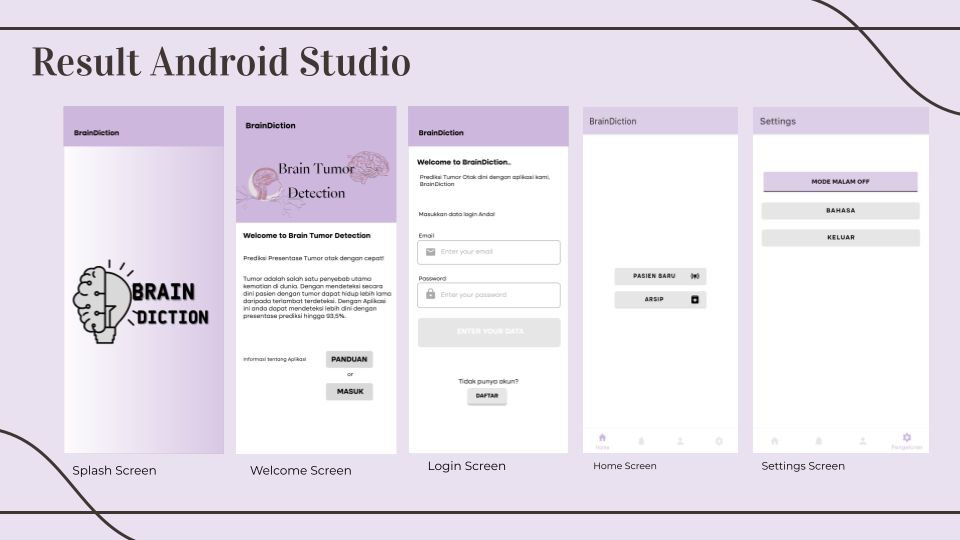
\includegraphics[scale=0.35]{./assets/loginhome}
	\caption{Tampilan login dan beranda aplikasi.}
\end{figure}
\begin{figure}[H]
	\centering
	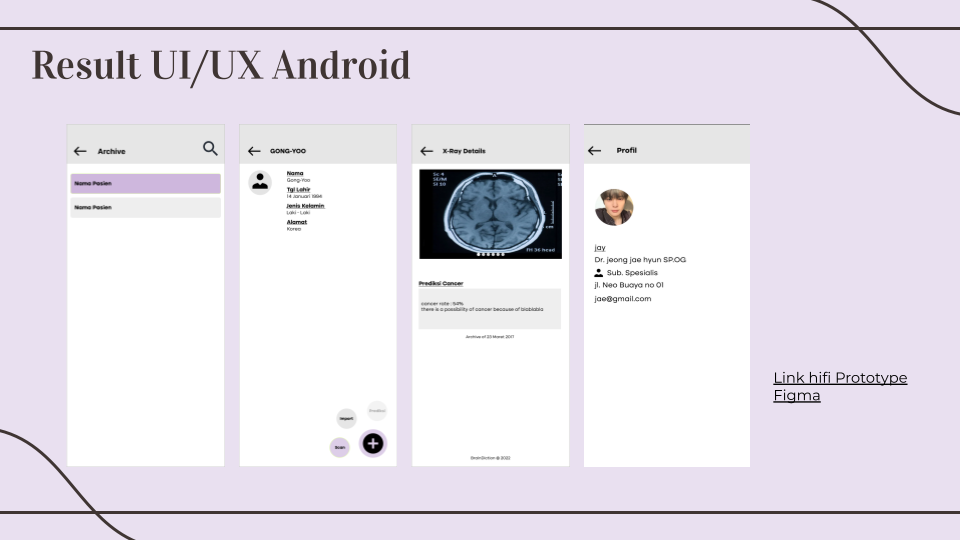
\includegraphics[scale=0.35]{./assets/predictionscreen}
	\caption{Tampilan prediksi aplikasi.}
\end{figure}
\subsection{Implementasi Materi}
Pada produk ini, kelompok kami mengimplementasikan seluruh elemen \textit{learning path} pada program Bangkit 2022:
\begin{enumerate}
	\item \textit{Cloud Computing} pada Google Cloud Platform
	\begin{itemize}
		\item Google Firebase Authentication
		\item Google Cloud Run untuk \textit{Backend} aplikasi dan \textit{machine learning}
		\item Google Cloud SQL untuk penyimpanan data pasien dan data prediksi
	\end{itemize}
	\item \textit{Machine Learning}
	\begin{itemize}
		\item Tensorflow untuk training model pendeteksi tumor otak
		\item Flask untuk \textit{Backend} penyalur dari Cloud Run ke model yang dihasilkan
	\end{itemize}
	\item \textit{Android Development}
	\begin{itemize}
		\item Kotlin dan Figma untuk pembuatan UI/UX aplikasi
	\end{itemize}
\end{enumerate}